\section{Reti Neurali Artificiali (ANN)}

\paragraph{Componenti principali del neurone biologico}
Per comprendere le ANN è indispensabile partire dalla loro ispirazione
biologica. I componenti principali di un neurone sono:
\begin{itemize}
    \item \textbf{Corpo cellulare (cell body / soma):} contiene il nucleo e il DNA.
    \item \textbf{Dendriti (dendrites):} strutture con migliaia di ramificazioni brevi, che captano segnali in ingresso.
    \item \textbf{Assone (axon):} struttura lunga che trasmette i segnali e si divide in terminazioni.
\end{itemize}

Il comportamento del neurone si articola in tre fasi:
\begin{enumerate}
    \item \textbf{INPUT:} ricezione di impulsi elettrici dai dendriti provenienti da altri neuroni.
    \item \textbf{ELABORAZIONE (Process):} i segnali vengono accumulati nel corpo cellulare.
    \item \textbf{OUTPUT:} se la somma supera una soglia, viene inviato un segnale lungo l'assone.
\end{enumerate}

\begin{figure}[H]
    \centering
    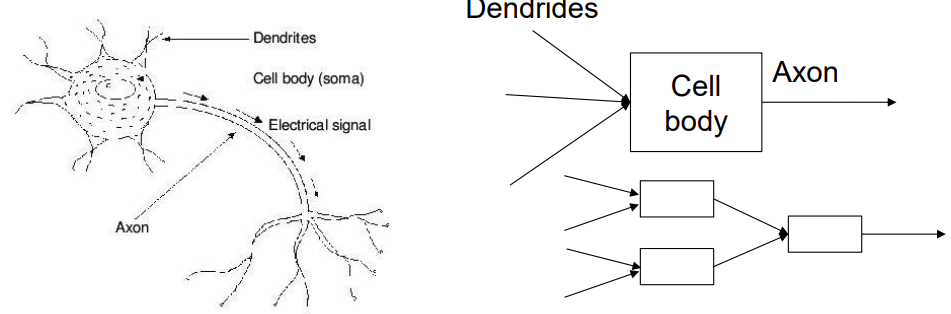
\includegraphics[width=0.8\textwidth]{img/neurone.png}
\end{figure}

\subsection{Artificial Neural Networks}

\paragraph{Percettrone}
In una ANN il \textbf{percettrone (Perceptron)} simula il neurone
biologico. Gli input $x_1, x_2, \dots, x_n$ vengono ponderati dai pesi
$w_1, w_2, \dots, w_n$ e sommati in un nodo centrale (corpo cellulare
artificiale). Il risultato passa attraverso una \textbf{funzione di
attivazione (Activation function)}, che determina l'output emulando la
soglia biologica.

\paragraph{Struttura a livelli}
I neuroni sono organizzati in tre tipi di livello:
\begin{itemize}
    \item \textbf{Input Layer:} riceve i dati grezzi.
    \item \textbf{Hidden Layer(s):} uno o più livelli nascosti intermedi.
    \item \textbf{Output Layer:} produce il risultato finale.
\end{itemize}

\begin{figure}[H]
    \centering
    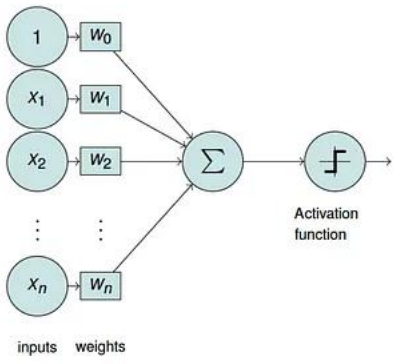
\includegraphics[width=0.4\textwidth]{img/perceptron.png}
\end{figure}

Una ANN con un singolo neurone e nessun livello nascosto equivale a una semplice \textbf{regressione logistica}.

\paragraph{Funzioni di attivazione comuni}
\begin{itemize}
    \item \textbf{Sigmoide:} $\sigma(z) = \dfrac{1}{1+e^{-z}}$ -- comprime l'output nell'intervallo $[0,1]$.
    \item \textbf{ReLU:} $R(z) = \max(0, z)$ -- lineare per valori positivi, zero per quelli negativi.
\end{itemize}

% ============================================================
\subsection{Meccanismo Operativo: Forward e Backward Pass}
% ============================================================

\subsubsection{Forward Pass: input through activation functions}

\paragraph{Calcolo per livello}
Il \textbf{passaggio in avanti (Forward Pass)} è la prima delle due fasi
operative. Per ogni livello si calcola prima il valore intermedio $Z$
come combinazione lineare degli input e dei pesi con il bias:
\[
Z = Wx + b
\]
Poi si applica la funzione di attivazione per ottenere l'attivazione del livello:
\[
A = \sigma(Z)
\]
Il processo si ripete a cascata fino all'output stimato $\hat{Y}$.

\begin{figure}[H]
    \centering
    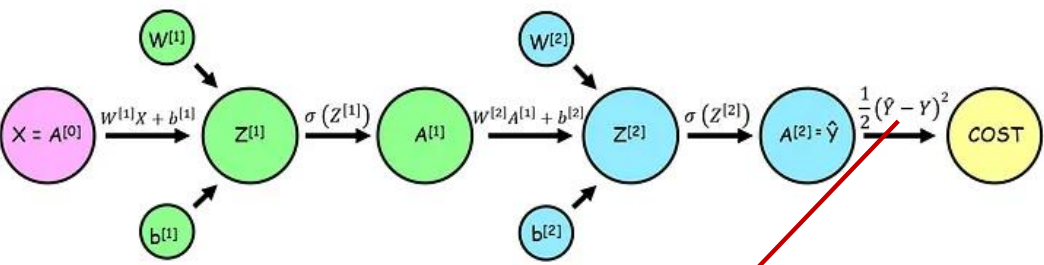
\includegraphics[width=0.9\textwidth]{img/forwardPass.png}
\end{figure}

\paragraph{Funzione di costo}
Per valutare la precisione si usa la \textbf{funzione di costo (Cost
function)}, tipicamente la metà dell'errore quadratico medio:
\[
J = \frac{1}{2}(Y - \hat{Y})^2
\]
L'obiettivo dell'addestramento è minimizzare $J$.

\subsubsection{Backward Pass: cost minimization}

\paragraph{Propagazione all'indietro}
Il \textbf{passaggio all'indietro (Backward Pass)} è finalizzato alla
minimizzazione del costo. La rete calcola il gradiente della funzione di
costo rispetto ai pesi, procedendo a ritroso dall'output verso
l'input. Tramite la \textbf{chain rule}, si determinano le derivate
parziali:
\[
\frac{\partial J}{\partial W} = \frac{\partial J}{\partial A}
\cdot \frac{\partial A}{\partial Z}
\cdot \frac{\partial Z}{\partial W}
\]
Analogamente si calcolano i gradienti per i bias e per i pesi dei livelli precedenti.

\begin{figure}[H]
    \centering
    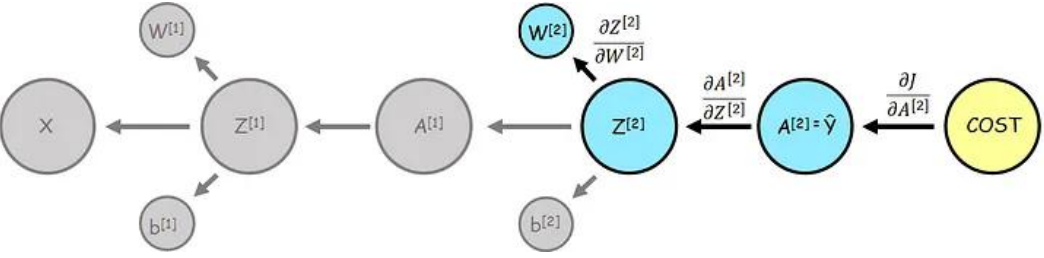
\includegraphics[width=0.9\textwidth]{img/backwardPass.png}
\end{figure}

\subsubsection{Weights update -- Aggiornamento dei pesi}

\paragraph{Discesa del gradiente}
Una volta ottenuti i gradienti, si procede con la \textbf{discesa del
gradiente (Gradient Descent)}. La regola di aggiornamento è:
\[
W_{\text{new}} = W_{\text{old}} - \alpha \frac{\partial J}{\partial W}
\]
dove $\alpha$ è il \textbf{learning rate (tasso di apprendimento)}. Lo stesso principio si applica al bias $b$.

\paragraph{Intuizione geometrica}
Graficamente: la funzione di costo è una curva parabolica. Se il
gradiente è positivo ci si muove a sinistra; se negativo, a destra --
puntando sempre verso il \textbf{minimo globale} dove il gradiente è
zero.

\begin{figure}[H]
    \centering
    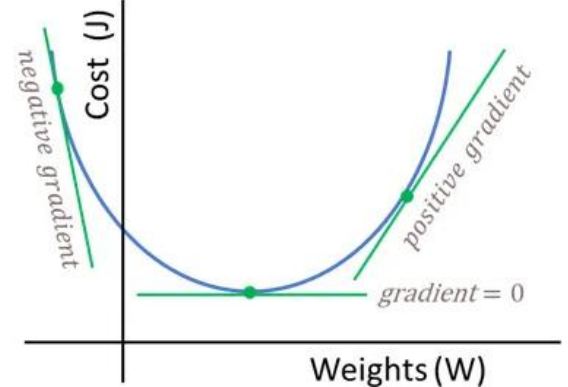
\includegraphics[width=0.5\textwidth]{img/gradientDesc.png}
\end{figure}

% ============================================================
\subsection{Deep Learning e Sizing}
% ============================================================

\subsubsection{Multiple Hidden Layers in cascade}

\paragraph{Shallow vs Deep}
Una rete \textit{non profonda (feedforward)} ha tipicamente un singolo
livello nascosto tra input e output. Una \textbf{Deep Neural Network} è
invece caratterizzata da molteplici livelli nascosti in cascata: la
complessità delle connessioni aumenta drasticamente passando da uno a
tre o più strati nascosti.

\begin{figure}[H]
    \centering
    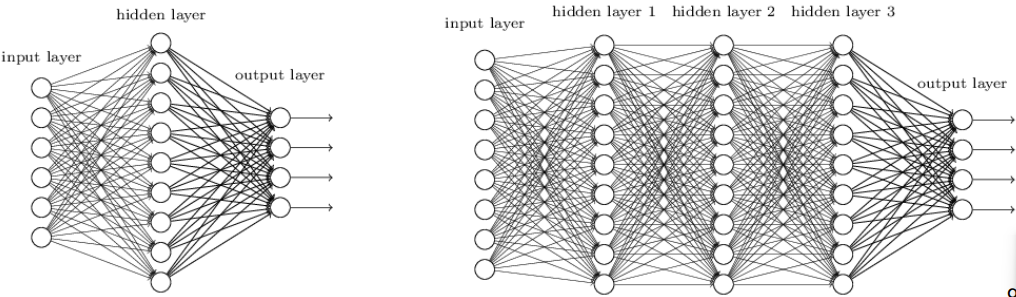
\includegraphics[width=0.8\textwidth]{img/complexityANN.png}
\end{figure}

\subsubsection{Complexity of ANNs}

\paragraph{Width e Depth}
La complessità si analizza su due dimensioni fondamentali:
\begin{itemize}
    \item \textbf{Larghezza (Width):} numero di neuroni per livello.
    \item \textbf{Profondità (Depth):} numero di livelli.
\end{itemize}
Più neuroni e più livelli $\Rightarrow$ maggiore capacità di apprendere
\textbf{caratteristiche latenti (latent characteristics)}, mappare
funzioni complesse ed estrarre feature di alto livello. Tuttavia ciò
porta a:
\begin{itemize}
    \item Maggiore complessità computazionale.
    \item Minore \textbf{spiegabilità (explainability)}: il modello diventa una ``scatola nera''.
    \item Maggiore capacità di fitting al dataset.
\end{itemize}

In termini di efficienza, addestrare modelli profondi può risultare più
efficiente rispetto a una rete a singolo strato con un numero massiccio
di neuroni.

\paragraph{Sizing ANNs -- Dimensionamento}
Non esiste un metodo analitico per il numero ottimale di livelli
nascosti: viene scelto \textbf{sperimentalmente} tramite tecniche come
la \textbf{cross-validazione}. Per il numero di neuroni per livello,
l'euristica suggerisce di impostarlo pari alla \textbf{media} tra i
neuroni dei livelli di input e output.

\paragraph{Basic Rules -- Regole empiriche}
\begin{itemize}
    \item Dataset linearmente separabile $\Rightarrow$ nessun livello nascosto necessario.
    \item Per molti problemi comuni, un singolo livello nascosto è sufficiente.
\end{itemize}

\subsubsection{Difficulties with single layer ANN}

Le reti molto larghe ma poco profonde (\textit{shallow}) eccellono nel
\textbf{memorizzare} i dati, ma mostrano carenze nella
\textbf{generalizzazione}. I livelli multipli, invece, apprendono
caratteristiche a diversi livelli di astrazione: le reti multistrato
performano decisamente meglio perché imparano matematicamente le
feature intermedie che collegano i dati grezzi alla classificazione di
alto livello finale.

\paragraph{Overfitting e Regolarizzazione}
Aumentare il numero di neuroni introduce più parametri da apprendere,
aumentando la probabilità di \textbf{overfitting}: reti troppo grandi
tendono a \textit{memorizzare} l'input piuttosto che generalizzare. Per
contrastarlo si adottano tecniche aggiuntive.

\begin{enumerate}
    \item Il \textbf{Dropout} consiste nel disattivare (\textit{congelare})
alcuni neuroni specifici degli hidden layer durante il training, con una
certa probabilità. Questo meccanismo:
\begin{itemize}
    \item Impedisce la co-dipendenza tra neuroni.
    \item Forza la rete a sviluppare percorsi ridondanti e robusti.
\end{itemize}
Durante la fase di \textbf{test}, tutti i neuroni sono attivi e gli
output vengono opportunamente \textbf{scalati} per mantenere la
coerenza con il comportamento in fase di addestramento.

    \item L'\textbf{Early Stopping} prevede il monitoraggio delle prestazioni su
un set di validazione. Quando la loss di validazione inizia a
peggiorare -- segno che la rete sta iniziando a sovra-adattarsi,
apprendendo rumore piuttosto che pattern generali -- il training viene
interrotto.
\end{enumerate}

% ============================================================
\subsection{Applicazioni e Risultati KDD'99}
% ============================================================

\subsubsection{Applications of ANNs to KDD'99}

Sul dataset \textbf{KDD'99} sono stati condotti due esperimenti:
\begin{enumerate}
    \item \textbf{Classificazione} tramite ANN multi-classe (Benign, DoS, Probe, R2L, U2R).
    \item \textbf{Anomaly detection} tramite autoencoder non supervisionato.
\end{enumerate}

\subsubsection{Classification performance of ANN}

\paragraph{Robust Scaling vs MinMax Scaling (no weights)}
Configurazione: Dropout=0.2, 2 livelli, 10 neuroni/livello.
\begin{itemize}
    \item \textbf{Robust Scaling (no weights):} buona separazione per
    BENIGN (162.486 corretti) e DoS (45.258), ma confusione tra PROBE e
    BENIGN (solo 2.443 PROBE corretti).
    \item \textbf{MinMax Scaling (no weights):} risultati simili con
    leggere variazioni; PROBE migliora leggermente (2.870 corretti).
    \item In entrambi i casi le classi minoritarie \textbf{R2L} e
    \textbf{U2R} mostrano tassi di rilevamento molto bassi o nulli.
\end{itemize}

\paragraph{Introduzione dei loss weights}
Con MinMax Scaling e \textbf{loss weights}, aumentando a 20 neuroni/livello:
\begin{itemize}
    \item Miglioramento rilevante per R2L (22 casi corretti rispetto ai valori trascurabili precedenti).
    \item Permangono errori di classificazione tra BENIGN e PROBE.
\end{itemize}

\paragraph{Effetto di 30 neuroni/livello}
Con 30 neuroni/livello (loss weights, MinMax): BENIGN rilevato con alta
precisione (160.875), DoS stabile (45.263). U2R rimane problematica:
solo 11 campioni corretti su un totale esiguo.

\paragraph{60 neuroni e configurazione asimmetrica (30+5)}
Aumentare fino a 60 neuroni non porta benefici lineari; in alcuni casi
aumenta la confusione su classi specifiche. La configurazione
asimmetrica 30+5 non risolve il problema delle classi minoritarie.

\paragraph{Classificazione gerarchica -- Hierarchical Classification (RF + ANN)}
L'approccio \textbf{ibrido gerarchico} (Random Forest + ANN) con
classificazione binaria finale (Benign vs Attack) raggiunge
un'accuratezza estremamente elevata:
\begin{itemize}
    \item 162.533 istanze benigne corrette; 62.417 attacchi corretti.
    \item Falsi positivi: 10; falsi negativi: 46.
\end{itemize}
Questo suggerisce che l'approccio ibrido e gerarchico supera le
limitazioni delle singole reti neurali shallow nella distinzione
macroscopica delle minacce.
